% This file was created by matlab2tikz.
%
%The latest updates can be retrieved from
%  http://www.mathworks.com/matlabcentral/fileexchange/22022-matlab2tikz-matlab2tikz
%where you can also make suggestions and rate matlab2tikz.
%
\definecolor{mycolor1}{rgb}{0.00000,0.44700,0.74100}%
\definecolor{mycolor2}{rgb}{0.85000,0.32500,0.09800}%
\definecolor{mycolor3}{rgb}{0.92900,0.69400,0.12500}%
\definecolor{mycolor4}{rgb}{0.49400,0.18400,0.55600}%
\definecolor{mycolor5}{rgb}{0.46600,0.67400,0.18800}%
%
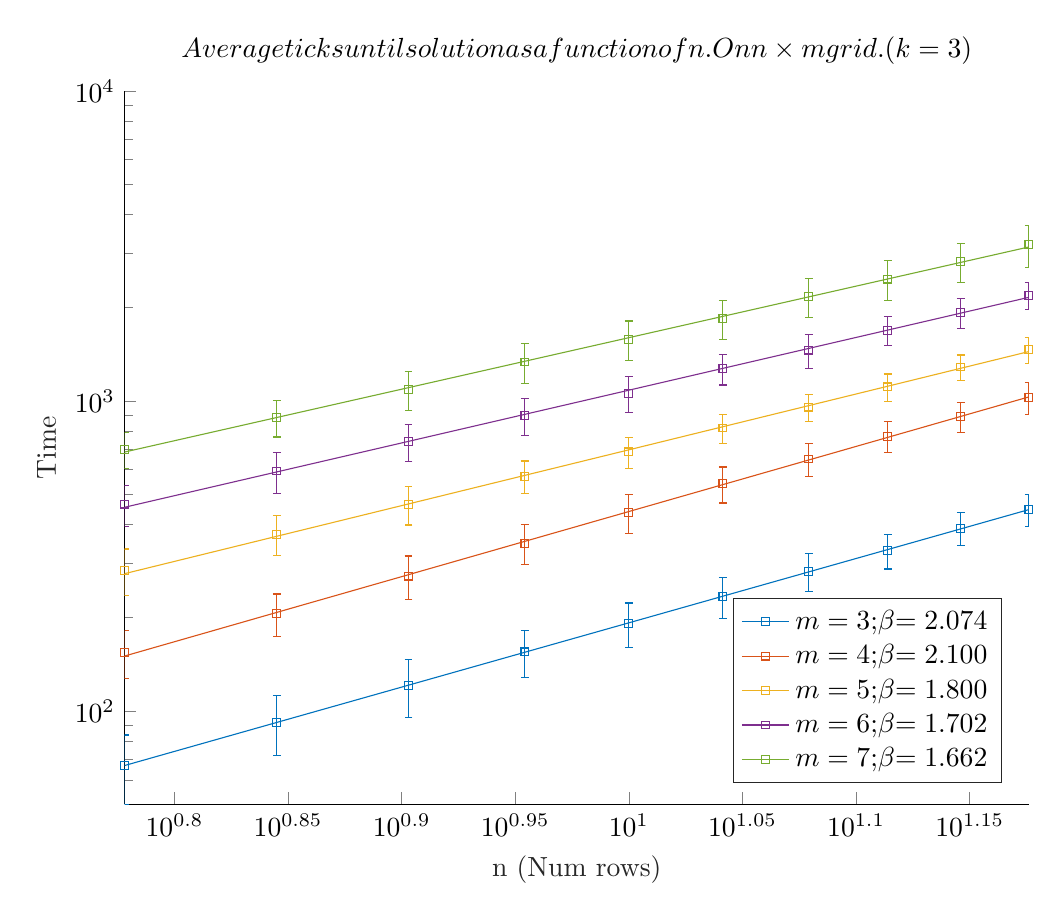
\begin{tikzpicture}

\begin{axis}[%
width=4.521in,
height=3.566in,
at={(0.758in,0.481in)},
scale only axis,
xmode=log,
xmin=6,
xmax=15,
xminorticks=true,
xlabel style={font=\color{white!15!black}},
xlabel={n (Num rows)},
ymode=log,
ymin=50.0788137681917,
ymax=10000,
yminorticks=true,
ylabel style={font=\color{white!15!black}},
ylabel={Time},
axis background/.style={fill=white},
title style={font=\bfseries},
title={$\text{Average ticks until solution as a function of n. On n }\times\text{ m grid. (k = 3)}$},
axis x line*=bottom,
axis y line*=left,
legend style={at={(0.97,0.03)}, anchor=south east, legend cell align=left, align=left, draw=white!15!black}
]
\addplot [color=mycolor1, draw=none, mark size=1.4pt, mark=square, mark options={solid, mycolor1}]
 plot [error bars/.cd, y dir = both, y explicit]
 table[row sep=crcr, y error plus index=2, y error minus index=3]{%
6	66.874	16.7951862318083	16.7951862318083\\
7	91.86	20.1232773818076	20.1232773818076\\
8	121.156	25.7125248053109	25.7125248053109\\
9	155.144	26.924731127582	26.924731127582\\
10	191.816	31.2520643646801	31.2520643646801\\
11	234.246	35.1346890800745	35.1346890800745\\
12	282.3	39.6902586696853	39.6902586696853\\
13	329.44	42.1596640706386	42.1596640706386\\
14	388.884	47.1406302677858	47.1406302677858\\
15	446.218	52.7492126469177	52.7492126469177\\
};
\addlegendentry{$\text{m = 3; }\beta\text{ = 2.074}$}

\addplot [color=mycolor1, forget plot]
  table[row sep=crcr]{%
6	66.7329894180365\\
7	91.8766110323815\\
8	121.197809622356\\
9	154.738327122566\\
10	192.535305394903\\
11	234.622231343625\\
12	281.02961481917\\
13	331.785491932466\\
14	386.91580932447\\
15	446.444724395747\\
};
\addplot [color=mycolor2, draw=none, mark size=1.4pt, mark=square, mark options={solid, mycolor2}]
 plot [error bars/.cd, y dir = both, y explicit]
 table[row sep=crcr, y error plus index=2, y error minus index=3]{%
6	154.3	27.0807816998504	27.0807816998504\\
7	206.298	32.2389188991127	32.2389188991127\\
8	272.258	44.0502927638985	44.0502927638985\\
9	347.434	51.0138654969989	51.0138654969989\\
10	436.504	62.9268906838903	62.9268906838903\\
11	540.682	71.912082233393	71.912082233393\\
12	650.282	79.7381139080881	79.7381139080881\\
13	768.704	88.1475147279004	88.1475147279004\\
14	891.216	97.8529291103283	97.8529291103283\\
15	1026.388	119.099701653143	119.099701653143\\
};
\addlegendentry{$\text{m = 4; }\beta\text{ = 2.100}$}

\addplot [color=mycolor2, forget plot]
  table[row sep=crcr]{%
6	150.496051019959\\
7	208.023199052796\\
8	275.35532570759\\
9	352.624563559889\\
10	439.948867312551\\
11	537.434891751671\\
12	645.1800621576\\
13	763.27411557715\\
14	891.80028037617\\
15	1030.83619984276\\
};
\addplot [color=mycolor3, draw=none, mark size=1.4pt, mark=square, mark options={solid, mycolor3}]
 plot [error bars/.cd, y dir = both, y explicit]
 table[row sep=crcr, y error plus index=2, y error minus index=3]{%
6	284.328	48.7171338880741	48.7171338880741\\
7	371.772	55.1817185317768	55.1817185317768\\
8	464.396	66.0276493975815	66.0276493975815\\
9	571.52	69.0452031654649	69.0452031654649\\
10	685.282	79.1400579576936	79.1400579576936\\
11	818.122	88.1637840705768	88.1637840705768\\
12	955.776	95.267736970156	95.267736970156\\
13	1110.83	111.388077043348	111.388077043348\\
14	1287.138	119.850186024805	119.850186024805\\
15	1463.198	138.808091148667	138.808091148667\\
};
\addlegendentry{$\text{m = 5; }\beta\text{ = 1.800}$}

\addplot [color=mycolor3, forget plot]
  table[row sep=crcr]{%
6	277.437951035728\\
7	366.15714199547\\
8	465.640534536811\\
9	575.603396684667\\
10	695.80103044191\\
11	826.019510759777\\
12	966.069250125542\\
13	1115.78035390938\\
14	1274.99916386753\\
15	1443.58561993373\\
};
\addplot [color=mycolor4, draw=none, mark size=1.4pt, mark=square, mark options={solid, mycolor4}]
 plot [error bars/.cd, y dir = both, y explicit]
 table[row sep=crcr, y error plus index=2, y error minus index=3]{%
6	464.716	70.7164831278532	70.7164831278532\\
7	594.304	90.0952045102929	90.0952045102929\\
8	739.322	100.819062099214	100.819062099214\\
9	896.734	125.010265085526	125.010265085526\\
10	1058.702	137.801741047315	137.801741047315\\
11	1271.748	145.253494454704	145.253494454704\\
12	1459.24	184.271262535407	184.271262535407\\
13	1689.216	182.836176614361	182.836176614361\\
14	1929.714	210.747890976641	210.747890976641\\
15	2190.392	216.00187025094	216.00187025094\\
};
\addlegendentry{$\text{m = 6; }\beta\text{ = 1.702}$}

\addplot [color=mycolor4, forget plot]
  table[row sep=crcr]{%
6	454.254291757122\\
7	590.489459816933\\
8	741.119388010655\\
9	905.579530229592\\
10	1083.39073955467\\
11	1274.13873643077\\
12	1477.46000294825\\
13	1693.03170532196\\
14	1920.56426295362\\
15	2159.79572407777\\
};
\addplot [color=mycolor5, draw=none, mark size=1.4pt, mark=square, mark options={solid, mycolor5}]
 plot [error bars/.cd, y dir = both, y explicit]
 table[row sep=crcr, y error plus index=2, y error minus index=3]{%
6	697.354	92.6912726639143	92.6912726639143\\
7	884.39	118.864508760545	118.864508760545\\
8	1089.346	156.090559642854	156.090559642854\\
9	1335.698	194.416455868903	194.416455868903\\
10	1580.916	230.879187764262	230.879187764262\\
11	1848.156	264.58948364156	264.58948364156\\
12	2173.03	317.878105694872	317.878105694872\\
13	2471.96	364.409004066158	364.409004066158\\
14	2822.684	408.018006380922	408.018006380922\\
15	3189.696	488.772376937275	488.772376937275\\
};
\addlegendentry{$\text{m = 7; }\beta\text{ = 1.662}$}

\addplot [color=mycolor5, forget plot]
  table[row sep=crcr]{%
6	684.632541812218\\
7	884.55209268777\\
8	1104.34889332325\\
9	1343.14231296048\\
10	1600.18867823284\\
11	1874.84784910076\\
12	2166.56036093062\\
13	2474.83116081348\\
14	2799.2176593341\\
15	3139.32071760085\\
};
\end{axis}
\end{tikzpicture}%